\clearpage
\section{5 СРАВНЕНИЕ С МОНОЛИТНОЙ ДЕТАЛИЗАЦИЕЙ}
\subsection*{Метод сравнения}
Для сравнения с монолитной детализацией, использующей монолитные лоды, был проведён следующий эксперимент: была настроена тестовая сцена, для этой сцены были проведены запуски реализованной упрощённой версии кластерного лоддирования и тривиального алгоритма монолитного лоддирования и измерены следующие параметры: количество кадров в секунду, количество треугольников, отправленных на растеризацию, количество растеризованных треугольников и количество запусков пиксельного шейдера.
Эти параметры характеризуют скорость выполнения отрисовки.

Также на тестовой сцене была составлена карта плотности треугольников для монолитного и кластерного лоддирования, для этого площадь каждого отображаемого треугольника была закодирована его цветом.
Эти карты показывают равномерность или неравномерность площади треугольников в разных частях экрана.

В качестве тестового меша была использована модель Thai Statue из The Stanford 3D Scanning Repository~\cite{StanfordRepo}, она содержит 10 млн. треугольников и 4~999~996 вершин.
Тестовая сцена содержит 64 объекта с таким исходным мешем.

Эксперимент проводился на ноутбуке с 16 ГБ оперативной памяти, видеокартой NVidia GeForce RTX 3060 Laptop GPU, процессором AMD Ryzen 7 5800H (3201 МГц, 8 физических ядер, 16 логических процессоров), разрешением монитора 2560 на 1440 и частотой обновления 165 Гц.
Приложение запускалось в режиме окна без рамки, развёрнутого на весь экран.

\subsection*{Проведение сравнения}
Для создания лодов был использован модификатор Decimate в Blender.
Размеры сгенерированных лодов приведены в таблице~\ref{tab:lod-sizes}.

\begin{table}[h]
    \centering
    \caption{Размеры лодов}

    \begin{tabular}{lrr}
        \hline \hline
        & Количество треугольников
        & Количество вершин \\ \hline
        LOD0 & 10 000 000 & 4 999 996 \\
        LOD1 &  1 000 000 &   499 996 \\
        LOD2 &    100 000 &    49 996 \\
        LOD3 &     10 000 &      4996 \\
        LOD4 &       1000 &       496 \\
        LOD5 &        100 &        46 \\
        LOD6 &         10 &        18 \\
        \hline \hline
    \end{tabular}

    \label{tab:lod-sizes}
\end{table}

При конвертации исходного меша в граф мешлетов для кластерной детализации получен граф с характеристиками, указанными в таблице~\ref{tab:graph-sizes}.

\begin{table}[h]
    \centering
    \caption{Граф мешлетов}

    \begin{tabular}{lr}
        \hline \hline
        Всего мешлетов    &    269 925 \\
        Истоков           &    104 167 \\
        Уникальных вершин &  6 166 095 \\
        Индексов          & 19 782 880 \\
        Всего примитивов  & 24 616 574 \\
        \hline \hline
    \end{tabular}

    \label{tab:graph-sizes}
\end{table}

% В процессе сравнения также была опробован метод отрисовки мешлетов без двойной индексации --- с разворачиванием массива вершин так, чтобы одному мешлету соответствовали записанные подряд в памяти вершины, а не записанные подряд в памяти индексы вершин.
% При использовании вершин размером 24 байта и индексов размером 4 байта это даёт массив вершин размером 452.8 мегабайта (474~789~120 байт), в сравнении с суммарным размером массивов вершин и индексов в 216.6 мегабайт (227~117~800 байт), т.е. дополнительные 109\% потребляемой памяти.
% Несмотря на это, подобный подход позволил увеличить производительность отрисовки, см. таблицу~\ref{tab:fps}.

На рисунке~\ref{fig:comparison-0} приведён скриншот выполнения с наивысшей точностью --- остальные режимы исполнения настраиваются так, чтобы визуальные отличия с этим режимом были минимальны.
На рисунках~\ref{fig:comparison-mono} и~\ref{fig:comparison-cluster} приведены скриншоты выполнения в режиме монолитного и кластерного лоддирования.
Визуальная разница этих режимов с наивысшим разрешением несущественна.

\begin{figure}[H]
    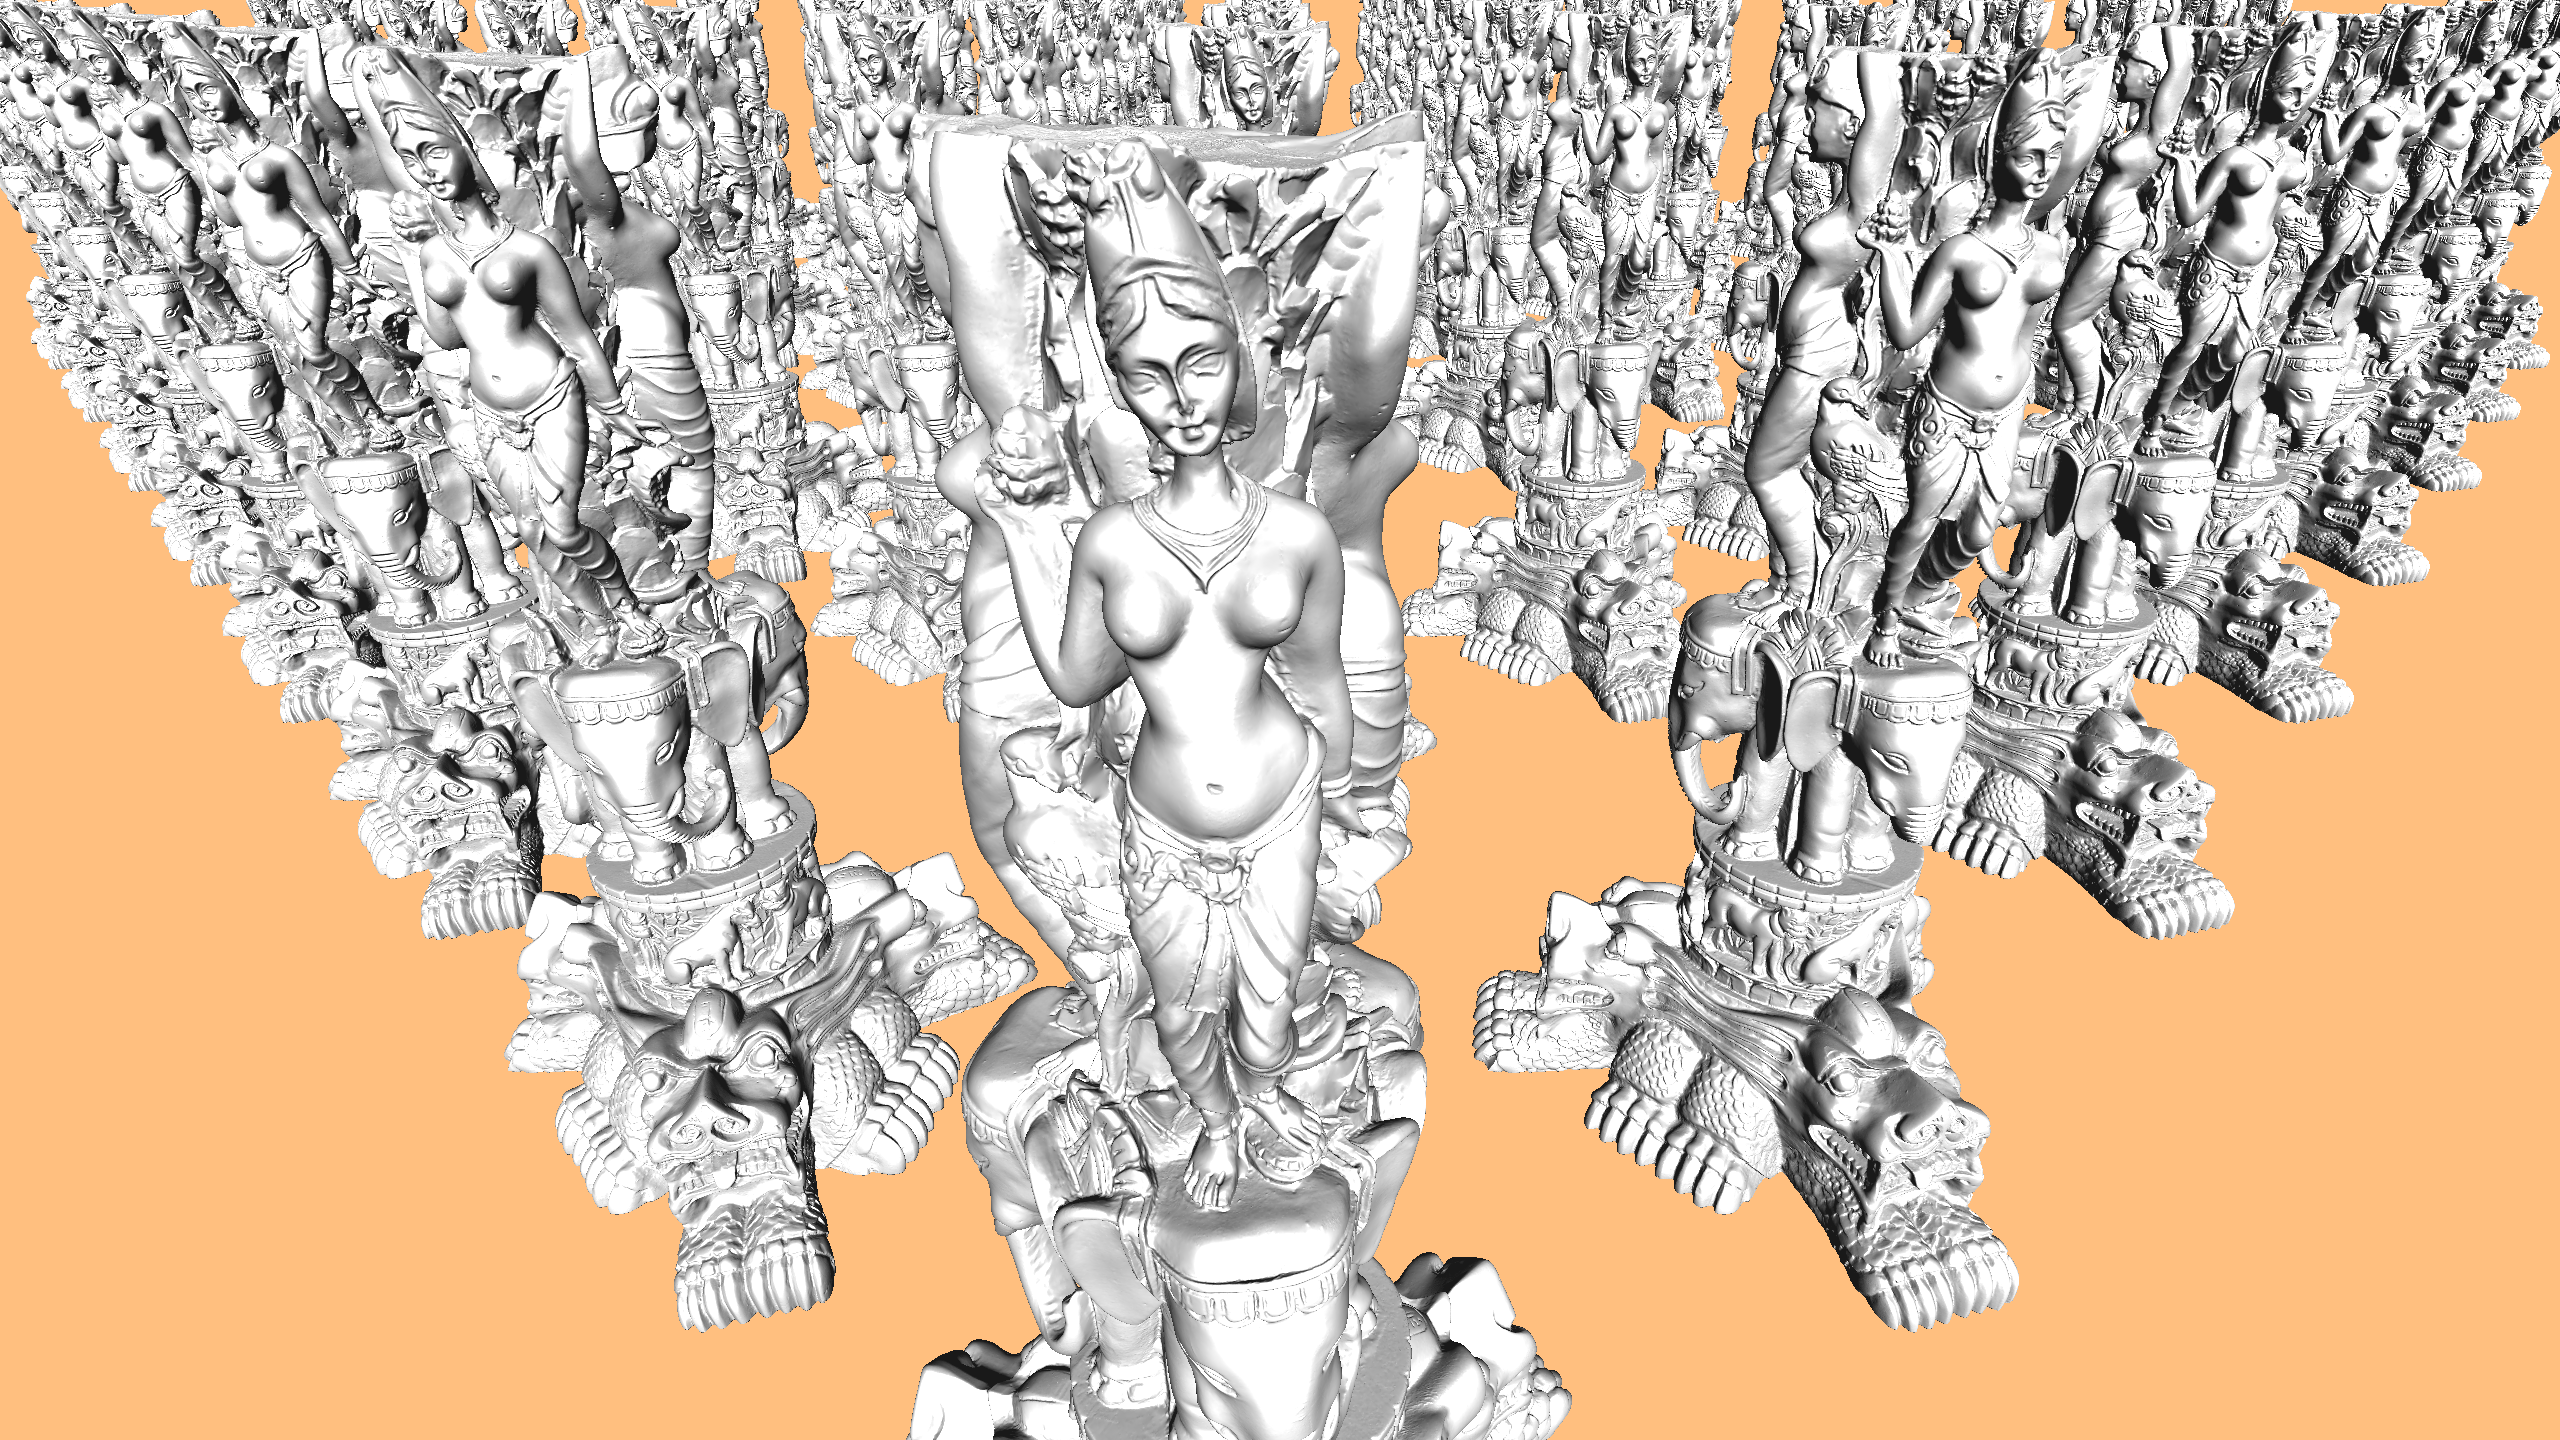
\includegraphics[width=\textwidth]{pics/comparison-0.png}
    \caption{Наивысшее разрешение, без лодов}
    \label{fig:comparison-0}
\end{figure}

\begin{figure}[H]
    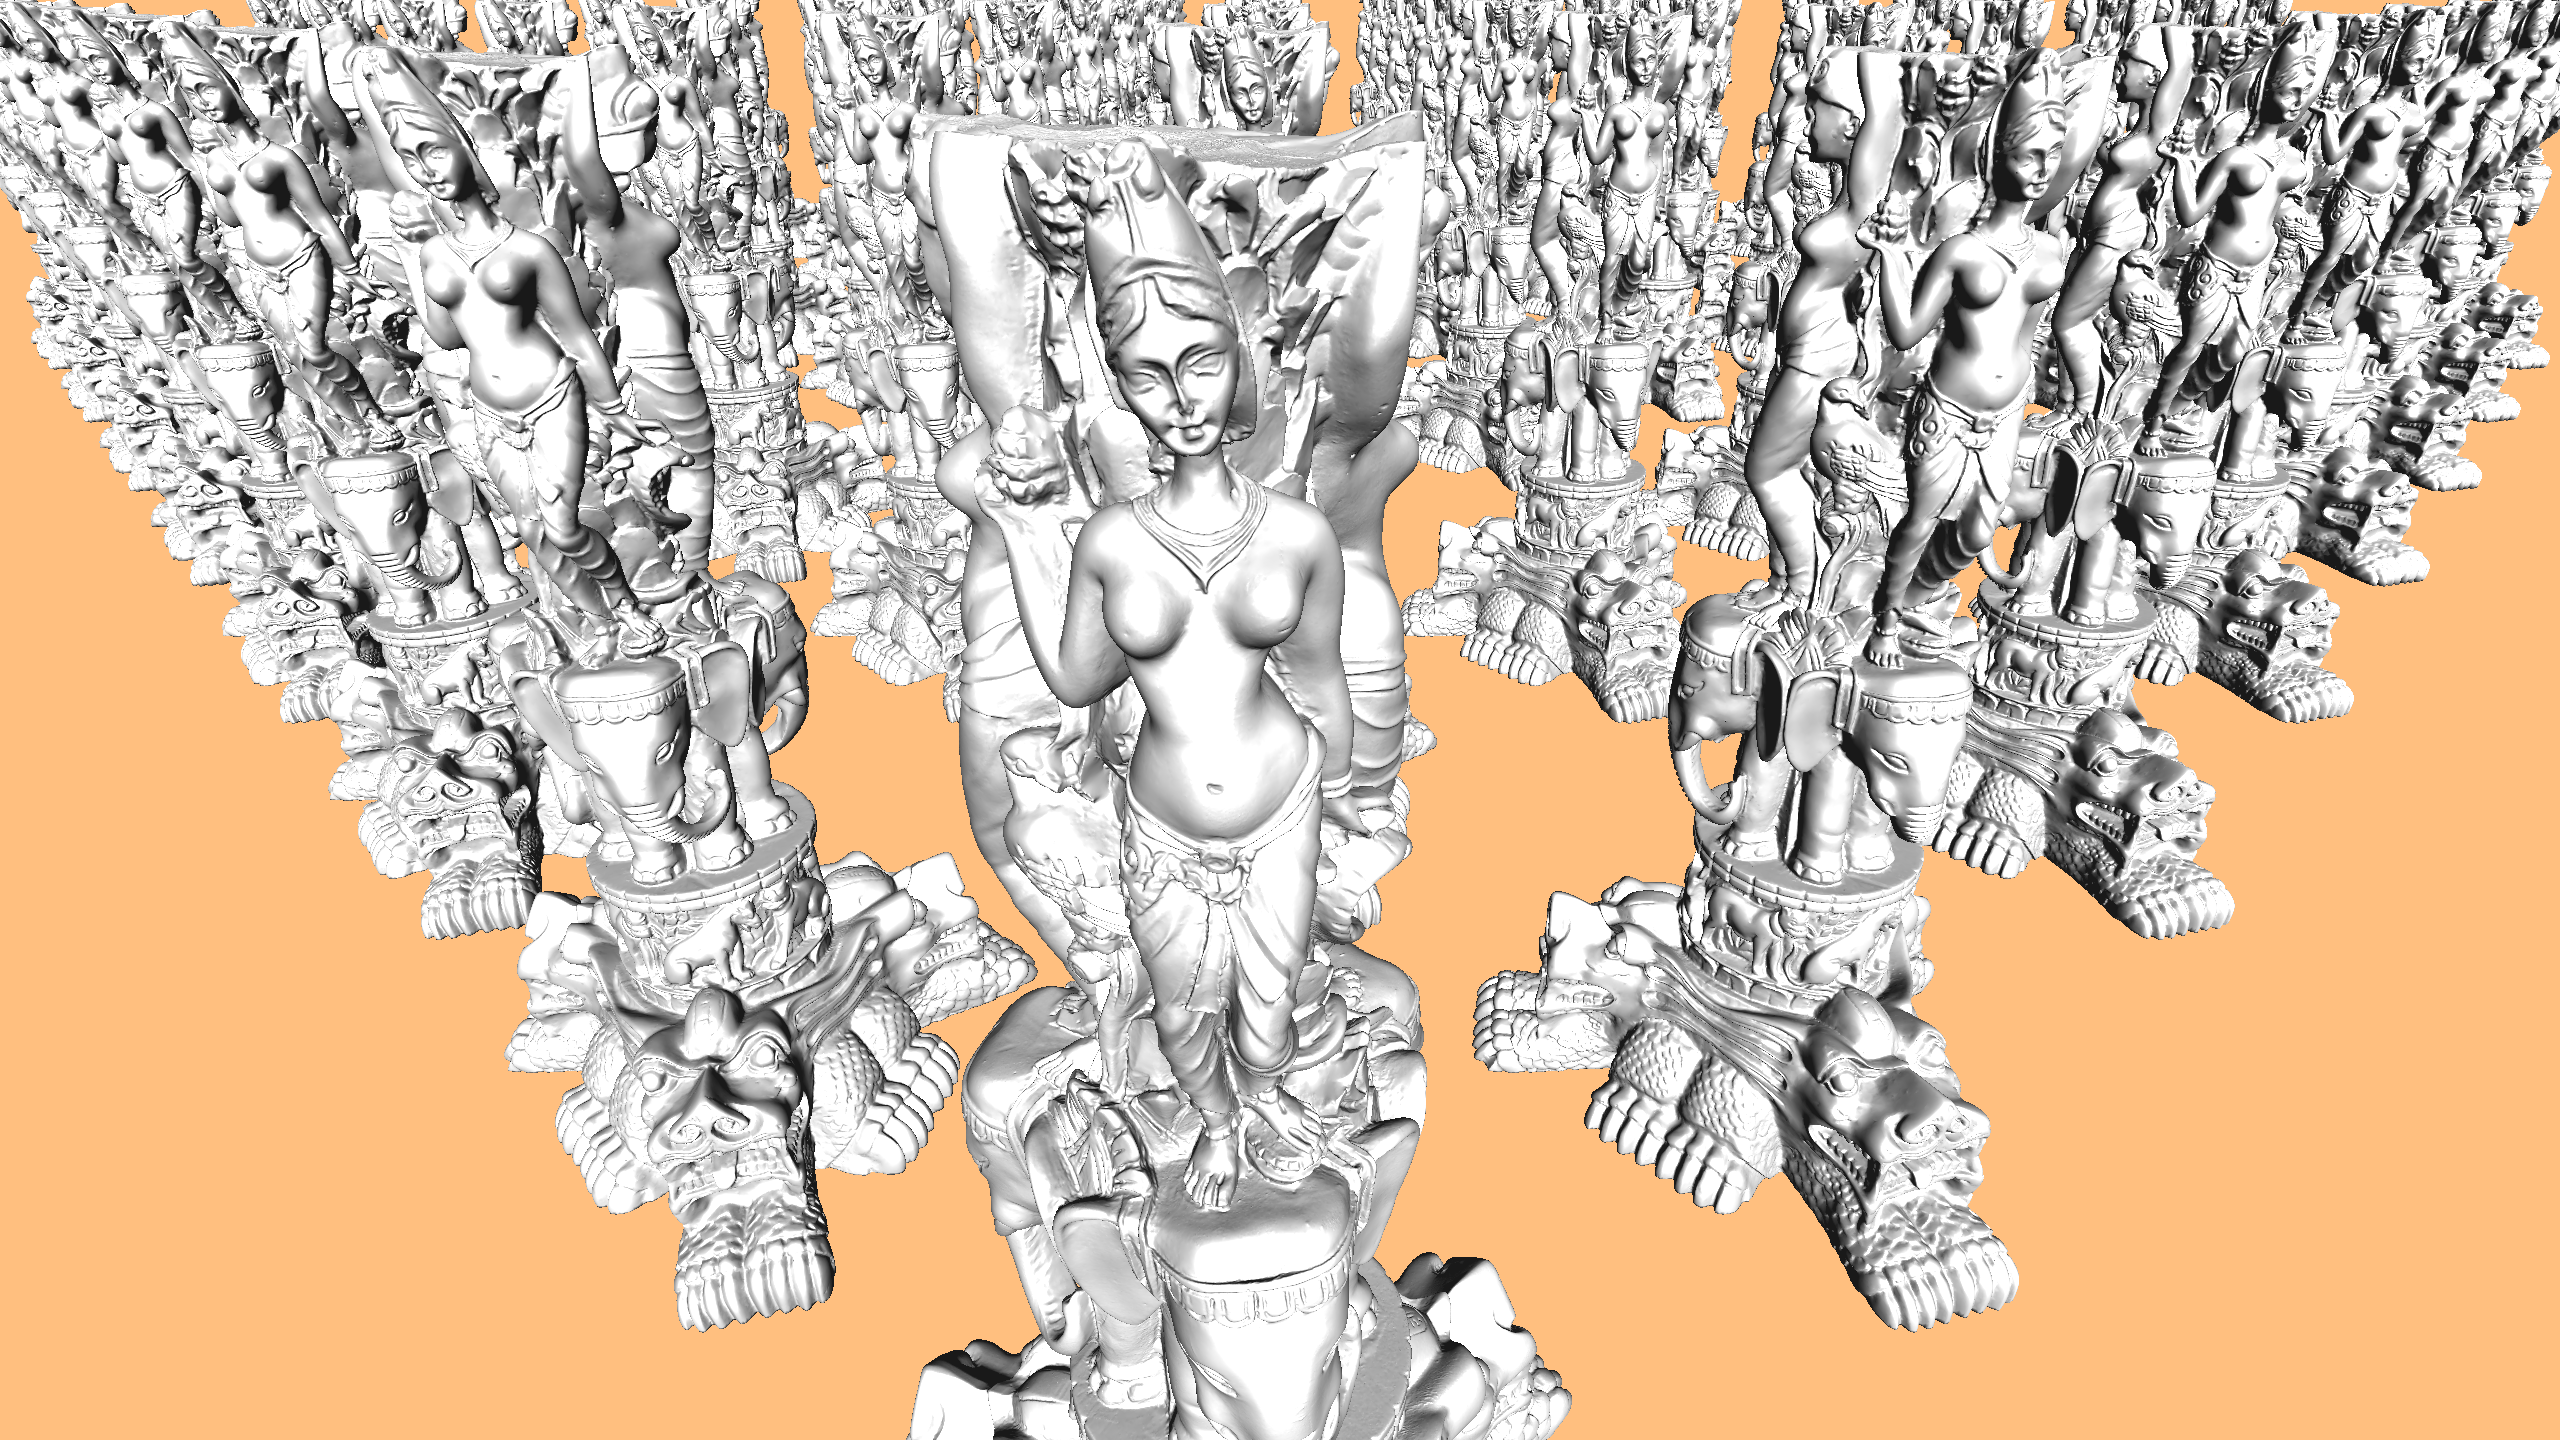
\includegraphics[width=\textwidth]{pics/comparison-mono.png}
    \caption{Монолитные лоды}
    \label{fig:comparison-mono}
\end{figure}

\begin{figure}[H]
    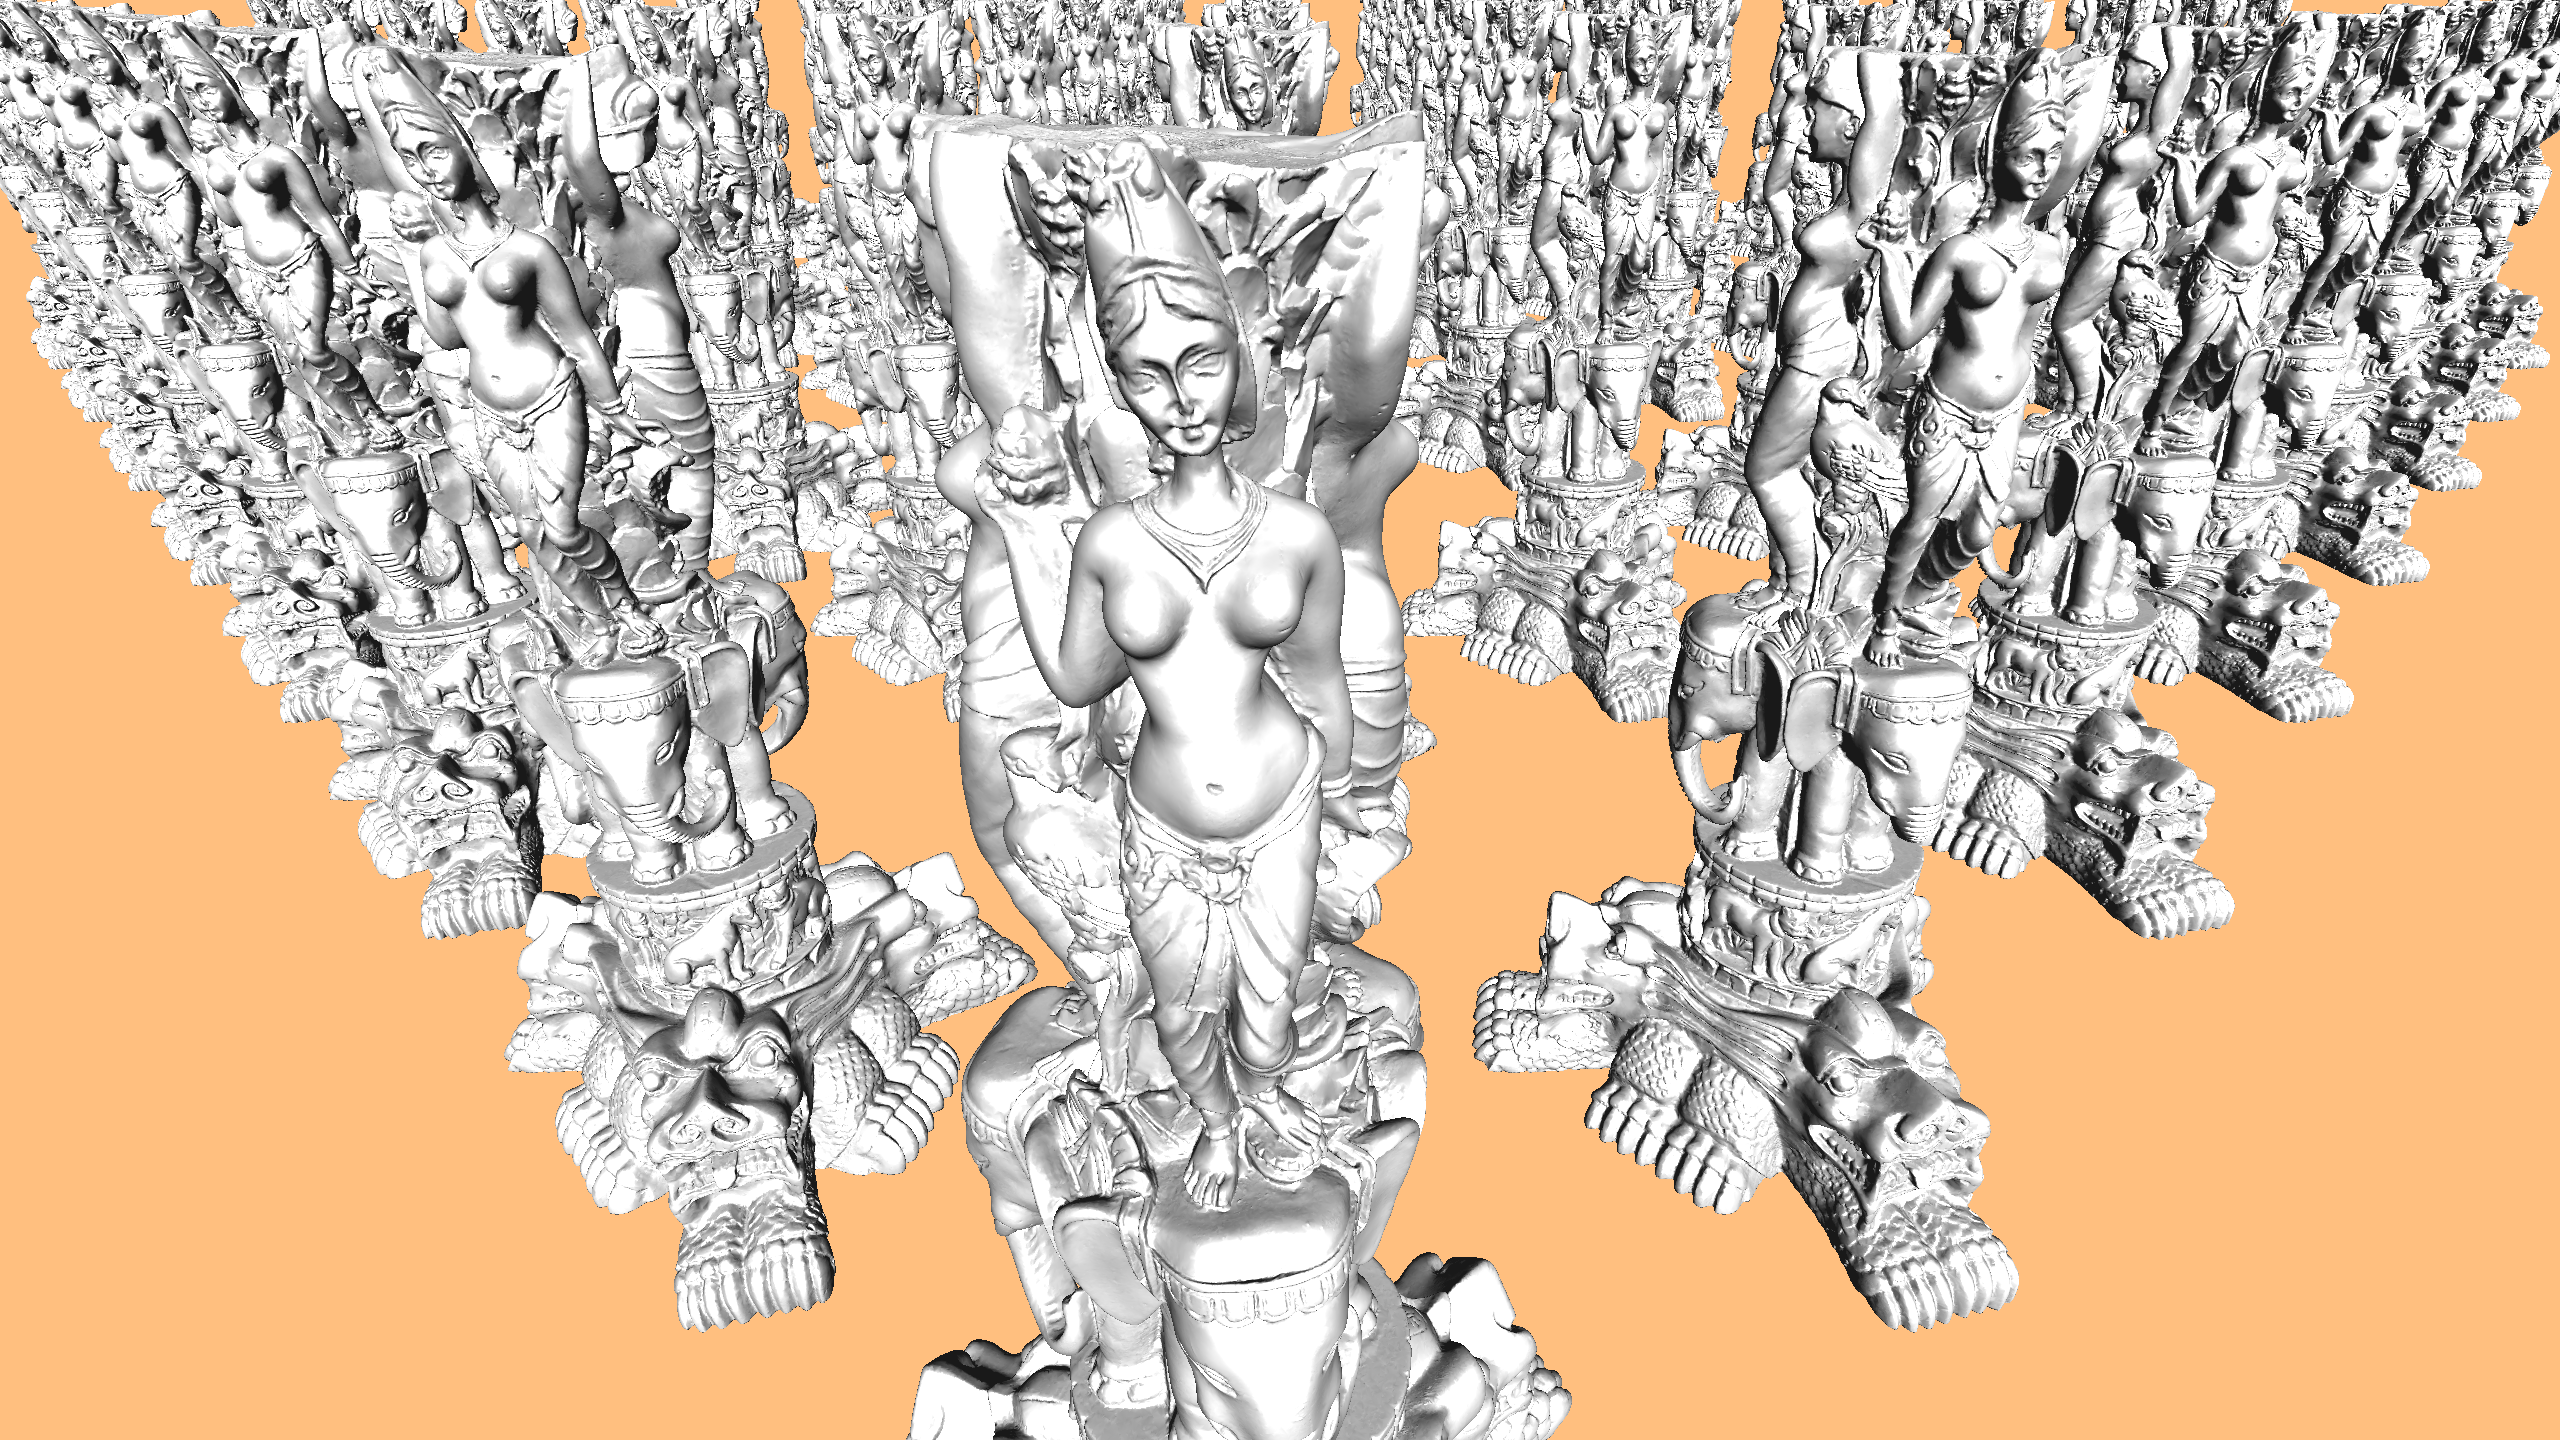
\includegraphics[width=\textwidth]{pics/comparison-cluster.png}
    \caption{Кластерные лоды}
    \label{fig:comparison-cluster}
\end{figure}

на рисунках~\ref{fig:heatmap-0}, \ref{fig:heatmap-mono} и~\ref{fig:heatmap-cluster} приведены карты площадей проекций отображаемых треугольников для наивысшей детализации, монолитных и кластерных лодов соответственно.
Красным цветом обозначены треугольники, проекции которых имеют площадь 1 пиксель, зелёным --- 3 пикселя, бирюзовым --- 7 пикселей, синим --- более 15 пикселей.

\begin{figure}[H]
    \includegraphics[width=\textwidth]{pics/heatmap-0.png}
    \caption{Площадь треугольников в наивысшем разрешении}
    \label{fig:heatmap-0}
\end{figure}

\begin{figure}[H]
    \includegraphics[width=\textwidth]{pics/heatmap-mono.png}
    \caption{Площадь треугольников монолитных лодов}
    \label{fig:heatmap-mono}
\end{figure}

\begin{figure}[H]
    \includegraphics[width=\textwidth]{pics/heatmap-cluster.png}
    \caption{Площадь треугольников кластерных лодов}
    \label{fig:heatmap-cluster}
\end{figure}

Рисунок~\ref{fig:heatmap-0} показывает, что наивысшее разрешение сильно избыточно для всех объектов, кроме ближайшего к камере, и можно сэкономить вычислительное время, уменьшив детализацию.
Рисунки~\ref{fig:heatmap-cluster} и~\ref{fig:heatmap-mono} показывают, что с помощью кластерных лодов удалось добиться более равномерной площади проекций треугольников, чем с помощью монолитных лодов.
При этом концентрация малых треугольников на большом удалении от камеры показывает, что оценка, на основании которой производится выбор мешлетов, пока недостаточно точна, и нужно искать способы её улучшить.

В таблице~\ref{tab:cmp} приведены результаты измерений.

\begin{table}[h]
    \centering
    \caption{Сравнение производительности}

    \begin{tabular}{lrrrr}
        \hline \hline
        Тип отрисовки
        & FPS
        & Отправлено
        & Растеризовано
        & Пикселей \\ \hline
        Наивысшее разрешение
        & 5.4
        & 640 000 000
        & 613 914 980
        & 2 880 524 \\
        Монолитные лоды
        & \textbf{114.2}
        & 28 900 000
        & 25 871 716
        & 2 880 722 \\
        % Кластерные лоды
        % & 27.2
        % & 56 021 881
        % & 55 940 686
        % & 2 492 760 \\
        Кластерные лоды
        & 35.0
        & 58 677 326
        & 57 256 188
        & 2 901 182 \\
        \hline \hline
    \end{tabular}

    \label{tab:cmp}
\end{table}

% \begin{figure}[H]
%     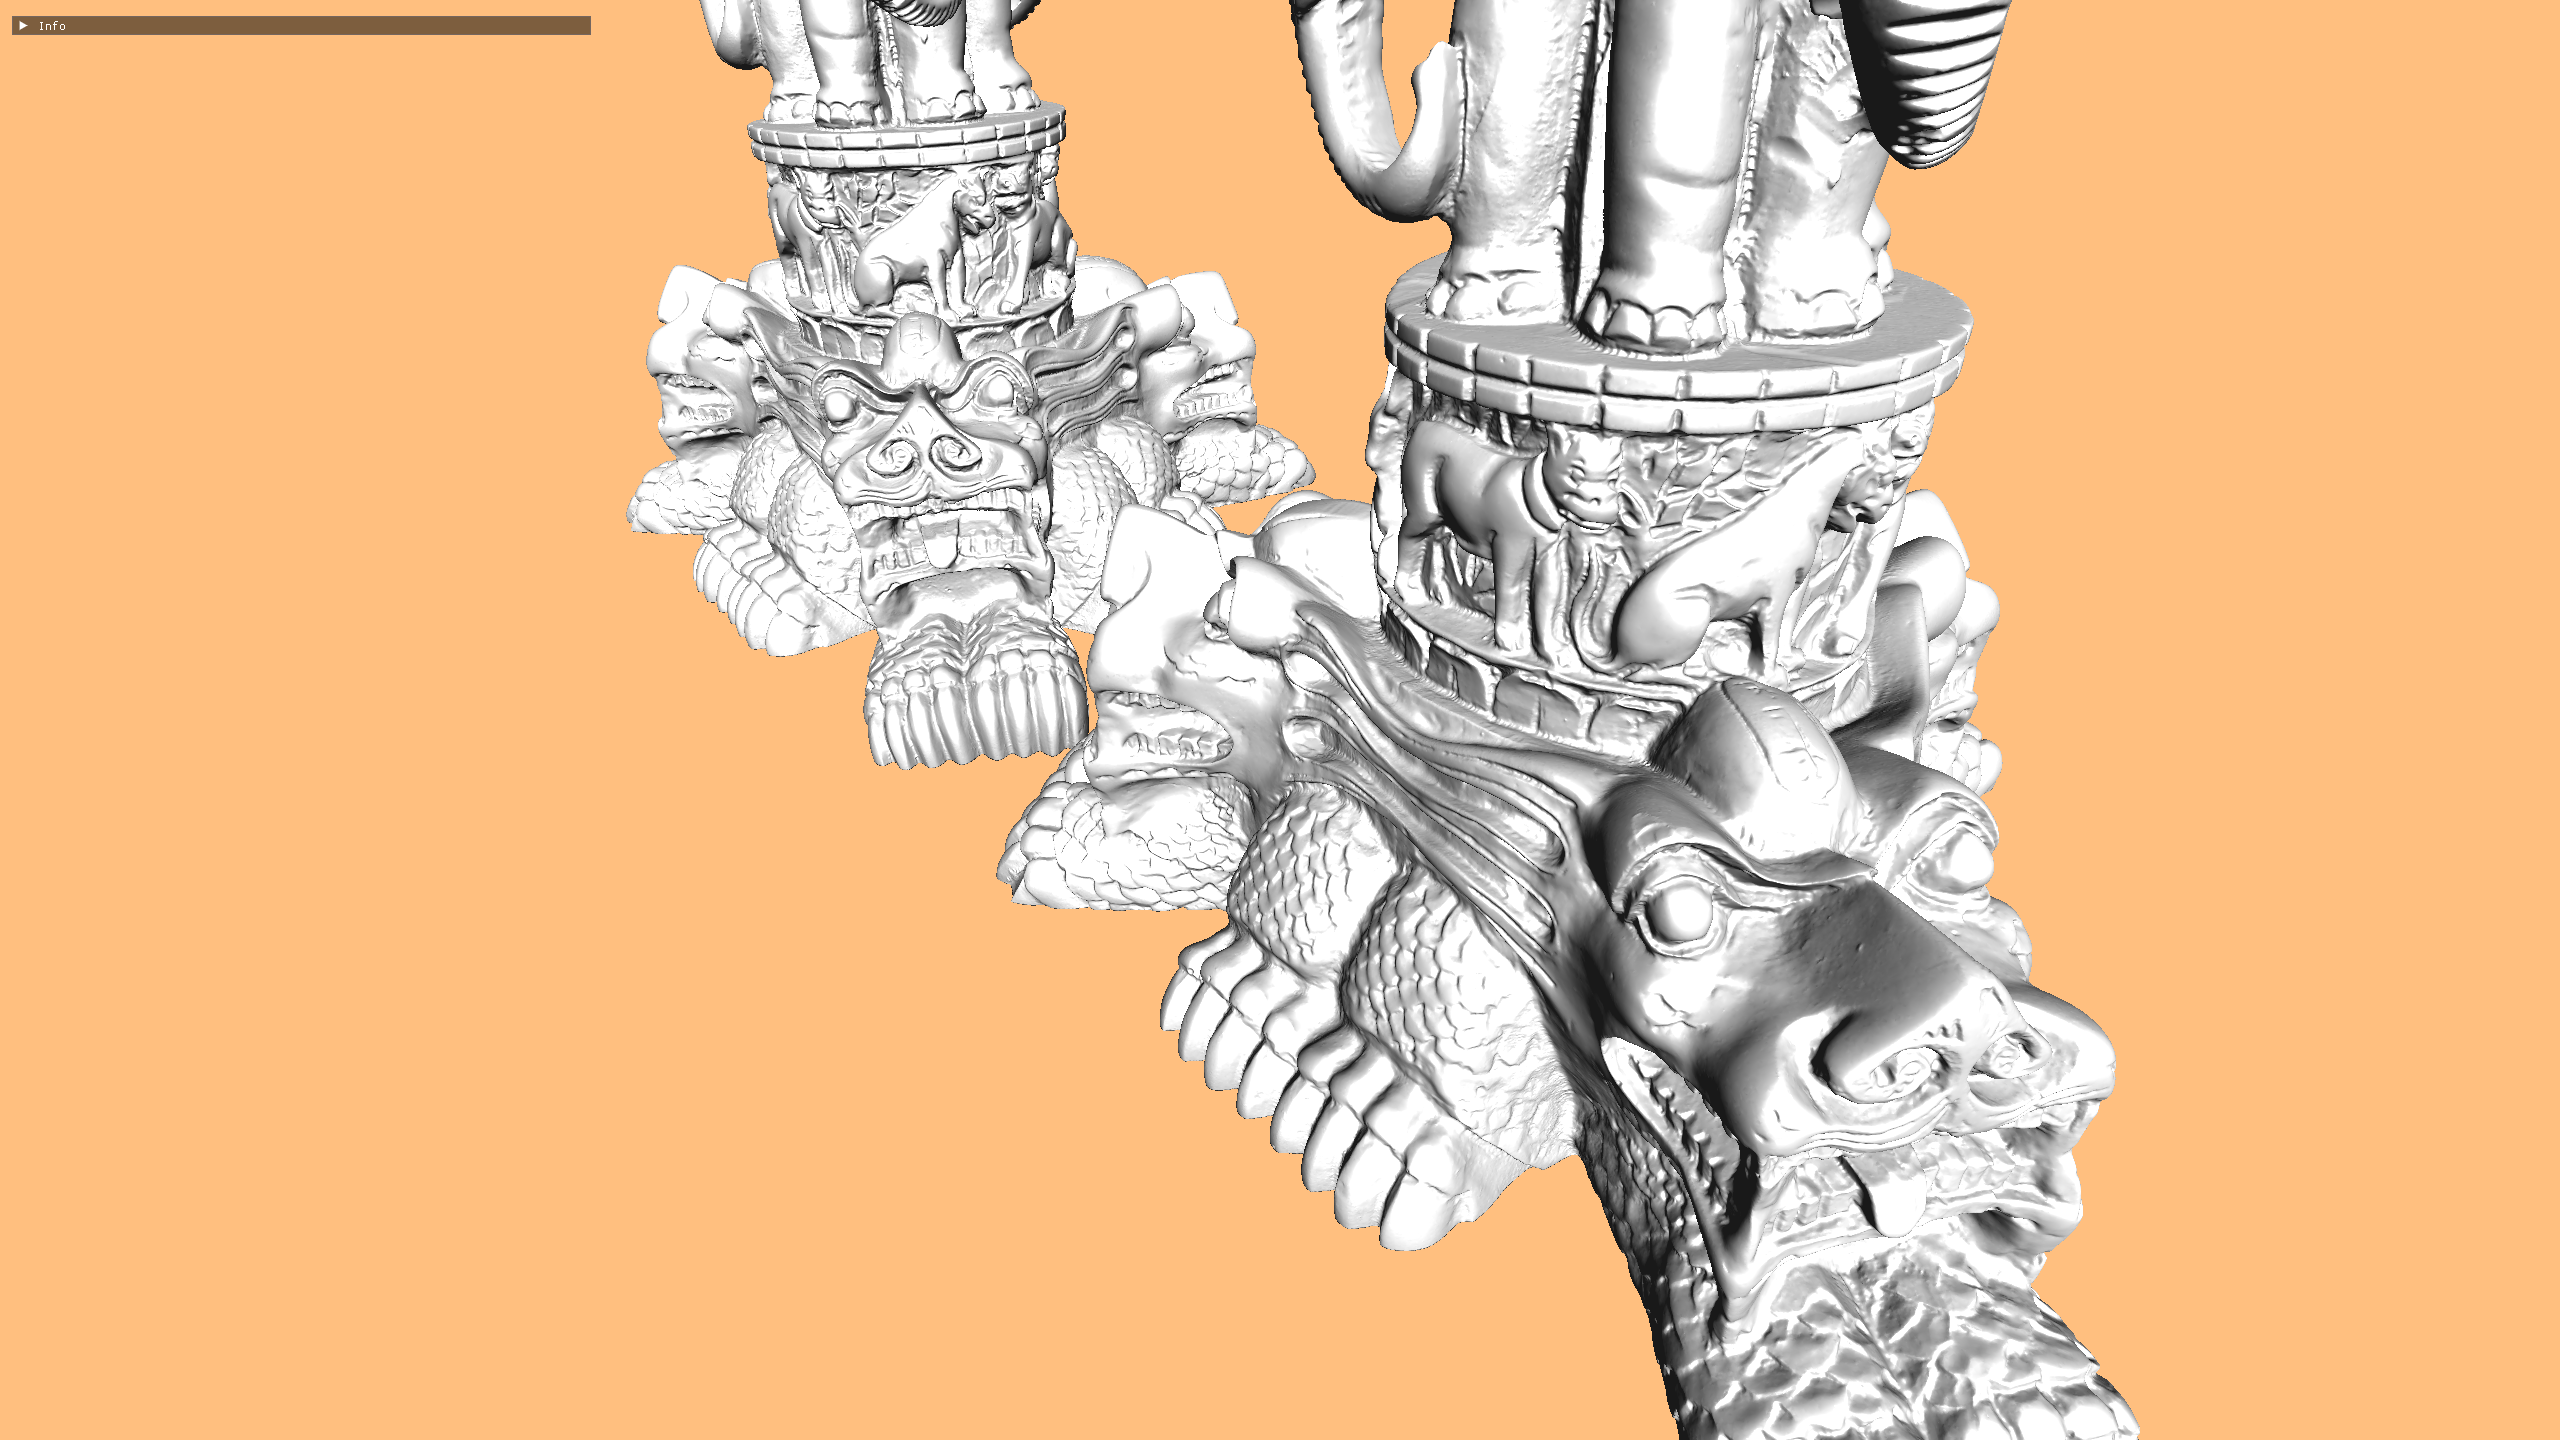
\includegraphics[width=\textwidth]{pics/mono-switch-1.png}
%     \caption{Переключение монолитных лодов, ракурс 1}
%     \label{fig:mono-switch-1}
% \end{figure}

% \begin{figure}[H]
%     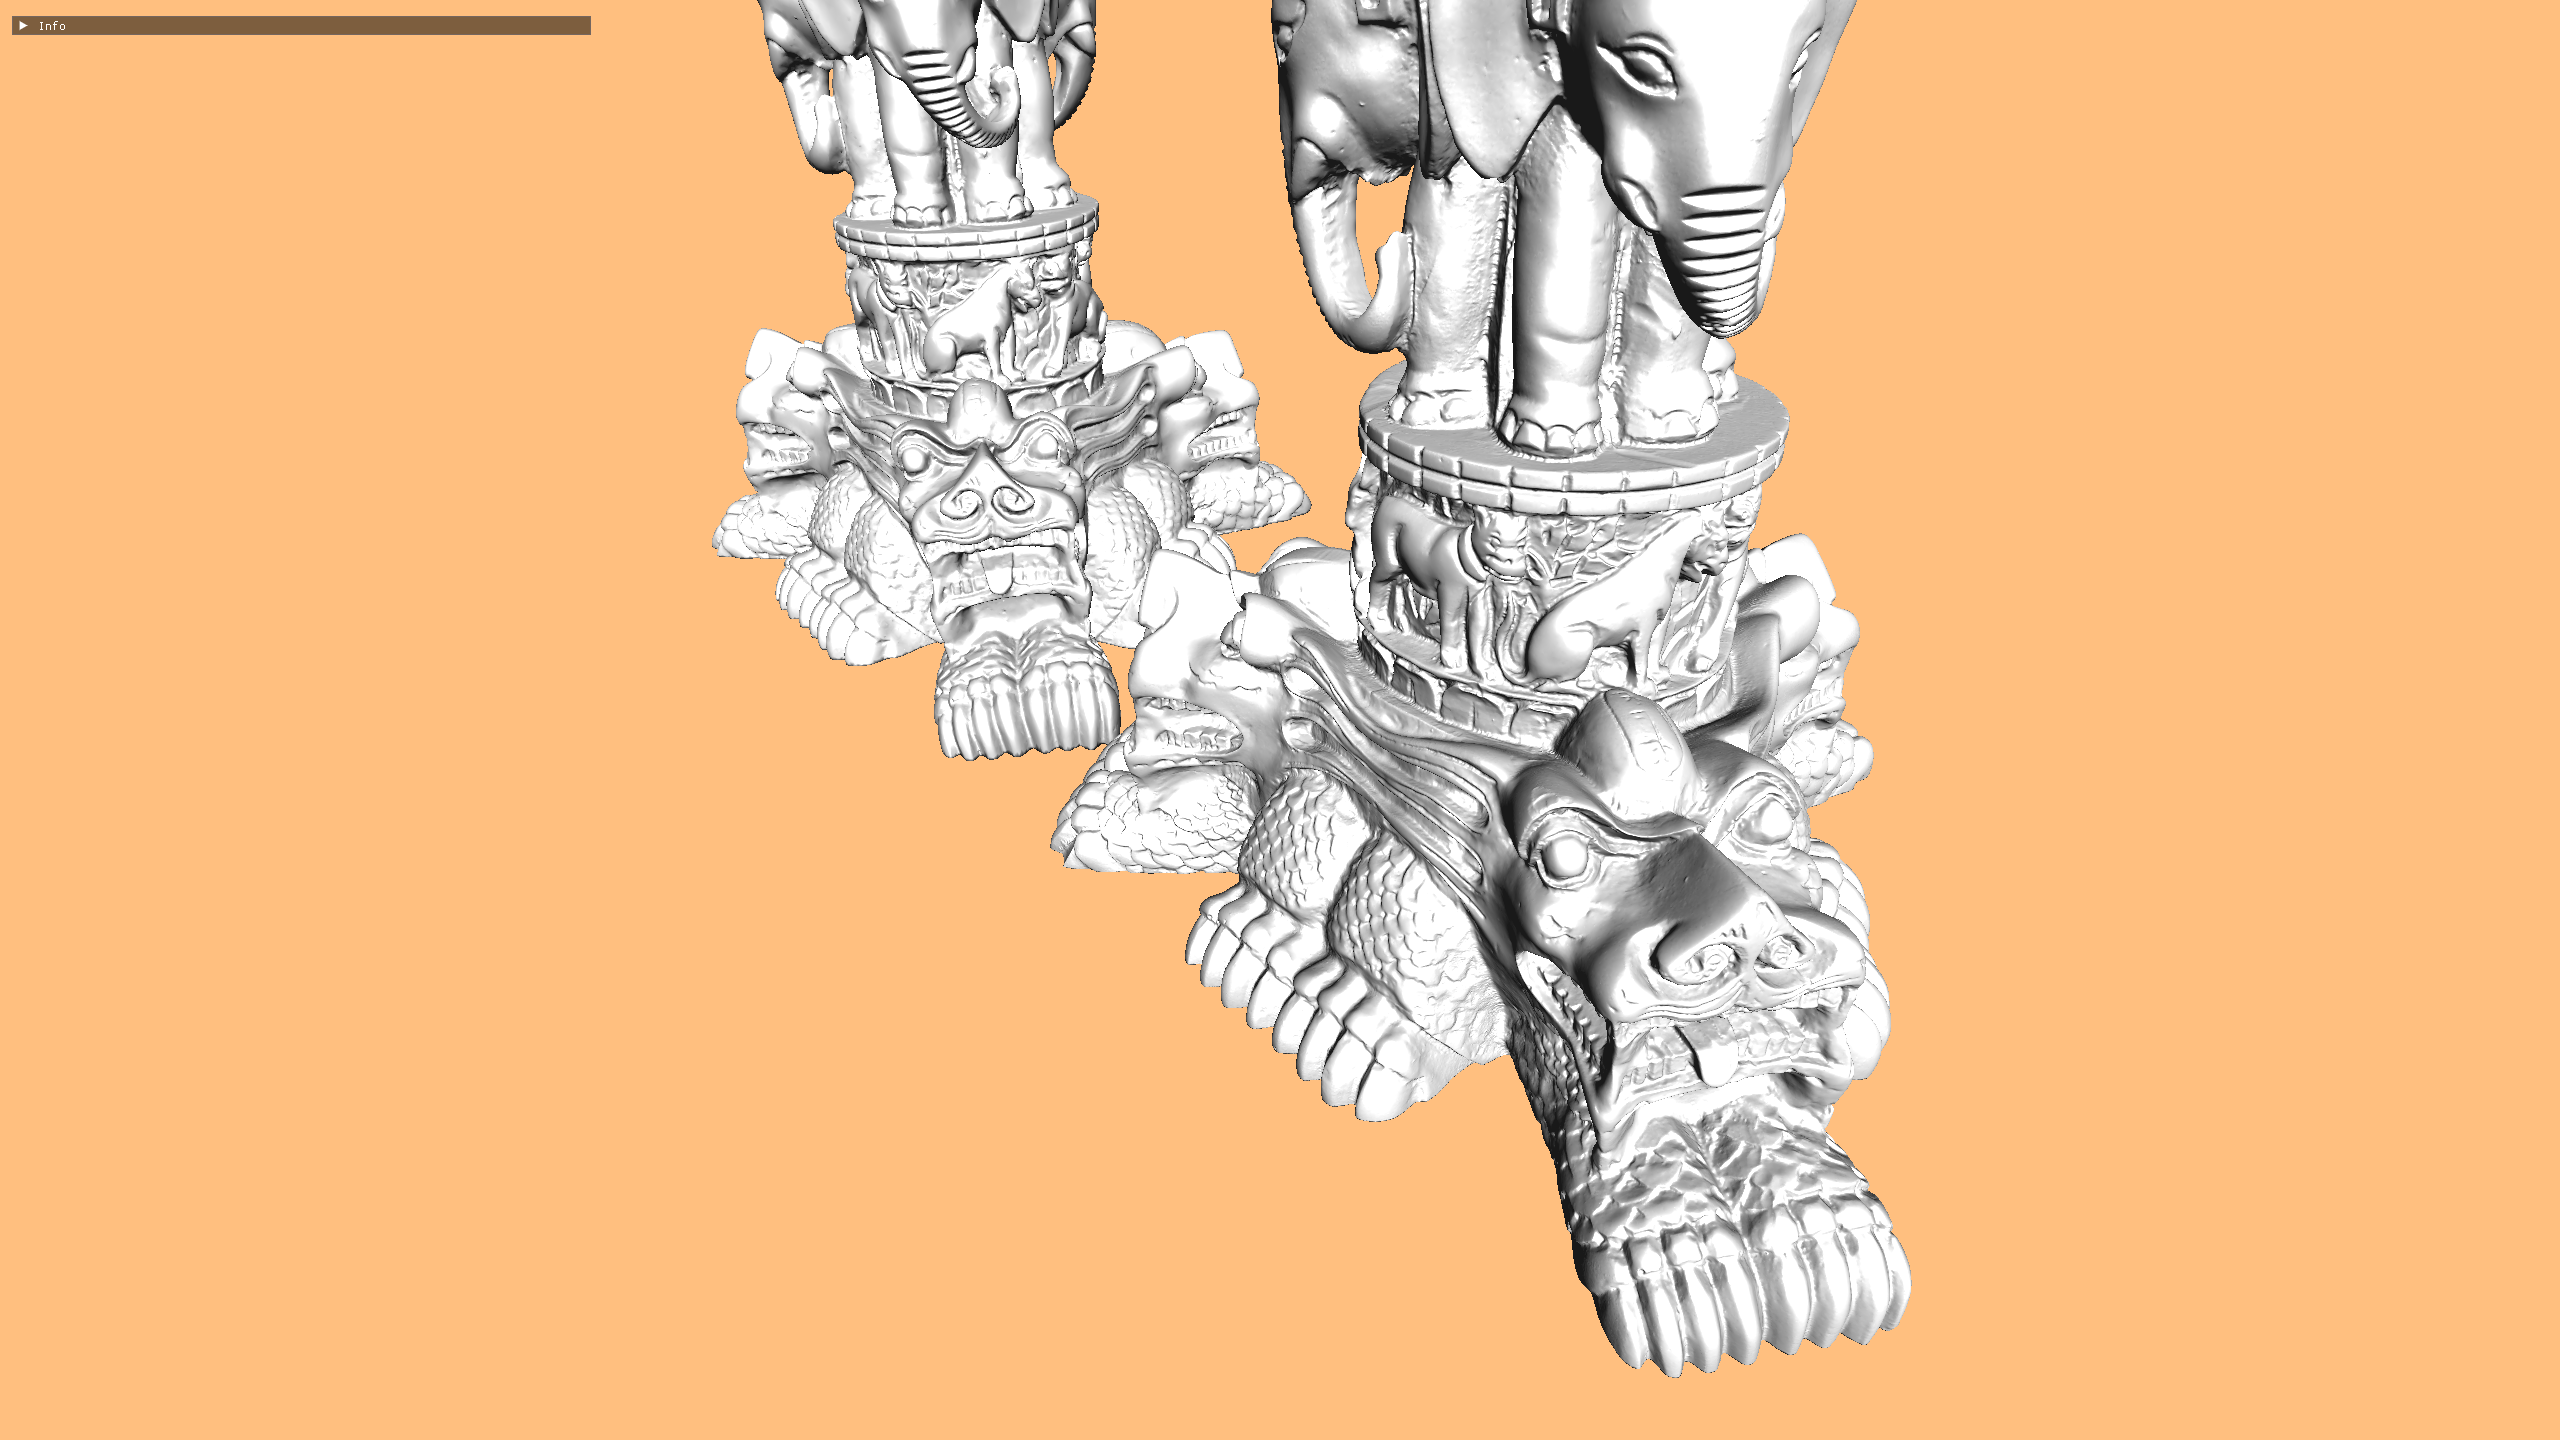
\includegraphics[width=\textwidth]{pics/mono-switch-2.png}
%     \caption{Переключение монолитных лодов, ракурс 2}
%     \label{fig:mono-switch-2}
% \end{figure}

% На рисунках~\ref{fig:mono-switch-1} и~\ref{fig:mono-switch-2} виден момент переключения монолитных лодов, кластерные лоды призваны избежать видимость такого переключения.

\subsection*{Заключение главы}
Сравнение с тривиальным алгоритмом монолитного лоддирования показало, что полученная реализация технологии процедурного кластерного видозависимого лоддирования пока сущетсвенно проигрывает в производительности, достигая только 31\% частоты кадров.
Для исправления этого в дальнейших работах предлагается исследовать те оптимизации, предложенные в главе 3, которые не были реализованы в данной работе.
